
% Include LaTeX packages
\documentclass[conference]{styles/acmsiggraph}
\usepackage{comment} % enables the use of multi-line comments (\ifx \fi)
\usepackage{fullpage}
\usepackage{enumitem}
\usepackage{amsmath,amsthm,amssymb}
\usepackage{listings}
\usepackage{graphicx}
\usepackage{etoolbox}
\usepackage{verbatim}
\usepackage{minted}
\usepackage[dvipsnames]{xcolor}
\usepackage{fancyvrb}
\usepackage{hyperref}
\usepackage{menukeys}
\usepackage{titlesec}
\usepackage{csquotes}
\usepackage{placeins}
\usepackage{algorithm} 
\usepackage{booktabs}
\usepackage{cases} 
\usepackage{algpseudocode}
\usepackage{unicode-math}
\newcommand{\?}{\stackrel{?}{=}}
\renewcommand\qedsymbol{$\blacksquare$}

% Set additional LaTeX options
\setlength{\parskip}{.8mm}
\setcounter{MaxMatrixCols}{20}
\hypersetup{
	colorlinks=true,
	urlcolor=[rgb]{0.97,0,0.30},
	anchorcolor={0.97,0,0.30},
	linkcolor=black,
	filecolor=[rgb]{0.97,0,0.30},
}

% Define title, author, and affiliation information
\title{\huge PSET 5 \\ \LARGE {CS124: Data Structures and Algorithms \\ Prof. Mitzenmacher}}
\author{\Large Dhilan Ramaprasad \\ dhilanramaprasad@college.harvard.edu}
\pdfauthor{Student Name}

% Redefine \VerbatimInput
\RecustomVerbatimCommand{\VerbatimInput}{VerbatimInput}%
{fontsize=\footnotesize,
 %
 frame=lines, % top and bottom rule only
 framesep=2em, % separation between frame and text
 rulecolor=\color{Gray},
 %
 label=\fbox{\color{Black}\textbf{OUTPUT}},
 labelposition=topline,
 %
 commandchars=\|\(\), % escape character and argument delimiters for commands within the verbatim
 commentchar=* % comment character
}

% Set addditional formatting options
\titlespacing*{\section}{0pt}{5.5ex plus 1ex minus .2ex}{2ex}
\titlespacing*{\subsection}{0pt}{3ex}{2ex}
\setcounter{secnumdepth}{4}
\renewcommand\theparagraph{\thesubsubsection.\arabic{paragraph}}
\newcommand\subsubsubsection{\paragraph}

% Define a convenient norm symbol
\newcommand{\norm}[1]{\left\lVert#1\right\rVert}
\renewcommand{\vec}[1]{\mathbf{#1}}

% Define a macro for hiding answers
\newbool{hideanswers} \setbool{hideanswers}{false}
\newenvironment{answer}{}{}
\ifbool{hideanswers}{\AtBeginEnvironment{answer}{\comment} %
\AtEndEnvironment{answer}{\endcomment}}{}

% Define text formatting for points and normals
\newcommand{\points}[1]{\hfill \normalfont{(\textit{#1pts})}}
\newcommand{\pointsin}[1]{\normalfont{(\textit{#1pts})}}







%%%%%%%%%%%%%%%%%%%%%%%%%%%%%%%%%%%%%%%
%%%%%%%%%%%%%%%%%%%%%%%%%%%%%%%%%%%%%%%
%%%%%%%%%%%%%%%%%%%%%%%%%%%%%%%%%%%%%%%
%%%%%%%%%%%%%%%%%%%%%%%%%%%%%%%%%%%%%%%
%%%%%%%%%%%%%%%%%%%%%%%%%%%%%%%%%%%%%%%

         %  START HERE  %

%%%%%%%%%%%%%%%%%%%%%%%%%%%%%%%%%%%%%%%
%%%%%%%%%%%%%%%%%%%%%%%%%%%%%%%%%%%%%%%
%%%%%%%%%%%%%%%%%%%%%%%%%%%%%%%%%%%%%%%
%%%%%%%%%%%%%%%%%%%%%%%%%%%%%%%%%%%%%%%
%%%%%%%%%%%%%%%%%%%%%%%%%%%%%%%%%%%%%%%

\begin{document}
\maketitle

\textbf{Collaborator}: No one :( \\
\textbf{Others:} A little advice from Phil \& Benny \\
\\ \\
I haven't been to Esther/Amy's office hours in a long time.  I miss going to their office hours :( \\
I haven't been to Rachel/Rose's section in a long time.  I miss going to their section :( \\

Sometimes, I, uh, even, uh, like, miss Professor Mitzenmacher :( \\

I don't miss Piazza.

\newpage

\section{Random Hash}
%%%%%%%%%%%%%%%%%%
%   Question #1  %
%%%%%%%%%%%%%%%%%%
Suppose each person gets a random hash value from $[1...n]$, show for at least $c_1 \sqrt{n}$ people in a room the probability no two have the same hash is less than or equal to $1/e$. \\

For $p$ people in a room and $n$ hash values:
\begin{align} \label{eq:Original}
    P(\text{distinct hashes}) = \prod_{i=0}^{p-1} \left ( 1- \frac{i}{n} \right )
\end{align}

Using the approximation $\left ( 1- \frac{i}{n} \right ) = e^{\frac{-i}{n}}$:
\begin{align} \label{eq:e_Approx}
    P(\text{distinct hashes}) = \prod_{i=0}^{p-1} e^{-\frac{i}{n}}
\end{align}

We can re-write these multiplied terms with exponents using exponent addition:
\begin{align}\label{eq:summative}
    P(\text{distinct hashes}) = e^{-\frac{1}{n} \cdot \sum_{i=0}^{p-1} i}
\end{align}

Ignoring the $i=0$ term---as it simply provides a factor of 1 in all Equations \ref{eq:Original}, \ref{eq:e_Approx}, and \ref{eq:summative}---we are presented with the following partial sum which is a \textit{triangular number}:
$$\sum_{i=1}^{p-1} i = \frac{(p-1)(p-1 + 1)}{2} = \frac{(p-1)(p)}{2}$$

Now, given that the probability is at most $1/e$ (as provided in PSET spec), we find the following:
\begin{align}\label{eq:LessThan}
    e^{-\frac{1}{n} \cdot \frac{(p-1)(p)}{2}} \leq \frac{1}{e}
\end{align}

Taking the natural log of both the left and right hand sides:
\begin{align}\label{eq:LessThan}
    -\frac{1}{n} \cdot \frac{(p-1)(p)}{2} & \leq -1 \\
    \frac{1}{n} \cdot \frac{(p-1)(p)}{2}  & \geq 1 \\
    \frac{p^2 - p}{2n}  & \geq 1 \\
    p^2 - p & \geq 2n \\
    p^2 - p - 2n & \geq 0 \\
\end{align}

Taking only the positive root of the quadratic:
\begin{align}
    p = \frac{-1 + \sqrt{1 + 8n}}{2}
\end{align}

Finally, substituting the given $c_1 \sqrt{n}$ for $p$, we find:
\begin{align}
    c_1 = \frac{-1 + \sqrt{1 + 8n}}{2\sqrt{n}}
\end{align}

\newpage

\section{Bloom Filters}
%%%%%%%%%%%%%%%%%%
%   Question #2  %
%%%%%%%%%%%%%%%%%%
\textbf{Setup}:
Given a $b$-bit counter, it is worth noting that its \enquote{max capacity} is $2^b - 1$.  That is, the counter of bit-width $b$ can count from $0$ to $2^b - 1$.  It overflows at $2^b$.

\subsection{Probability of overflow}
We are given $n$ elements to hash into $m$ locations using $k$ hash functions:

\begin{align} \label{eq:badProb}
    P(\text{overflow} \mid \text{bit width is } b) &= \sum_{i = 2^b}^{n} {n \choose i} \left( \frac{k}{m}\right )^i \left( 1 - \frac{k}{m} \right) ^{n-i}
\end{align}

The overflow probability shown above (Equation \ref{eq:badProb}) is not easily calculated via simulation for large $n$; however, it can be synonymously re-written to subtract away the cases in which overflow does not occur:
\begin{align} \label{eq:betterProb}
    P(\text{overflow} \mid \text{bit width is } b) &= 1 - \sum_{i = 0}^{2^b - 1} {n \choose i} \left( \frac{k}{m}\right )^i \left( 1 - \frac{k}{m} \right) ^{n-i}
\end{align}


\subsubsection{3-bit Counter}
\begin{align} \label{eq:betterProb}
    P(\text{overflow} \mid \text{bit width is } 3) &= 1 - \sum_{i = 0}^{7} {n \choose i} \left( \frac{k}{m}\right )^i \left( 1 - \frac{k}{m} \right) ^{n-i}
\end{align}


\subsubsection{4-bit Counter}
\begin{align} \label{eq:betterProb}
    P(\text{overflow} \mid \text{bit width is } 4) &= 1 - \sum_{i = 0}^{15} {n \choose i} \left( \frac{k}{m}\right )^i \left( 1 - \frac{k}{m} \right) ^{n-i}
\end{align}


\subsubsection{5-bit Counter}
\begin{align} \label{eq:betterProb}
    P(\text{overflow} \mid \text{bit width is } 5) &= 1 - \sum_{i = 0}^{31} {n \choose i} \left( \frac{k}{m}\right )^i \left( 1 - \frac{k}{m} \right) ^{n-i}
\end{align}

\subsection{Calculated Probabilities}
Given $n = 10^5$, $m = 10^6$, and $k = \lceil (m/n) \cdot \text{ln}2 \rceil$

% Table generated by Excel2LaTeX from sheet 'Sheet1'
\begin{table}[htbp]
  \centering
    \begin{tabular}{c|c}
    \multicolumn{1}{c}{Bit Width} & Probability of Overflow \\
    \midrule
    3     & 7.69E-07 \\
    4     & 8.19E-17 \\
    5     & 2.12E-41 \\
    \end{tabular}%
  \label{tab:bitWidth}%
  \caption{Counter Bit-widths v. Probability of Overflow}
\end{table}%

It is sensible to use a 4 bit counter as the probability of overflow is sufficiently small.  Additional gains are made with the 5 bit, but if you're resource constrained, it may be better to trade off the near negligible probability gains for less resource consumption.

\subsection{Code Excerpts}
I used three methods to solve this problem due to the precision needed for each successive value.  The first two were in python and last in Mathematica.\\

\textbf{Python Selection:}
\begin{minted}{python}
from scipy.special import comb
import numpy as np
import decimal

getcontext().prec = 100


def innerSum(b, n, m):
  k = np.ceil((m/n)*np.log(2))
  upperBound = 2**b
  summation = 0
  for i in range (0, upperBound):
    summation += Decimal(comb(n,i))*((Decimal(k)/m)**i)*((1-(Decimal(k)/m))**(n-i))
  return 1 - summation
  
threebit = 1 - innerSum(3, 10**5, 10**6)
fourbit = 1 - innerSum(4, 10**5, 10**6)
\end{minted}

\textbf{\\ \\Mathematica Selection:}
\begin{minted}{mma}
m = 10^6
n = 10^5
k = Ceiling[(m/n)*Log[2]]
N[Evaluate[
  1 - Sum[Binomial[n, i]*(k/m)^i (1 - k/m)^(n - i), {i, 0, 31}]]]
\end{minted}


\newpage

\section{Document Similarity}
%%%%%%%%%%%%%%%%%%
%   Question #3  %
%%%%%%%%%%%%%%%%%%
\textbf{Setup:}\\
Though it was unclear as to the representation of the \enquote{values} in the original sketch (i.e., the minimums of 84 permutations), the exact composition of these values did not play a role in further considerations of probability; nevertheless, knowledge of their structure could be useful in determining---at scale---whether collision probability (though seemingly low as seen in the proceeding calculations) is non-negligible.  In any case, I show my interpretation of the setup in Figure \ref{fig:similarity} below.

\begin{figure}[h!]
    \centering
    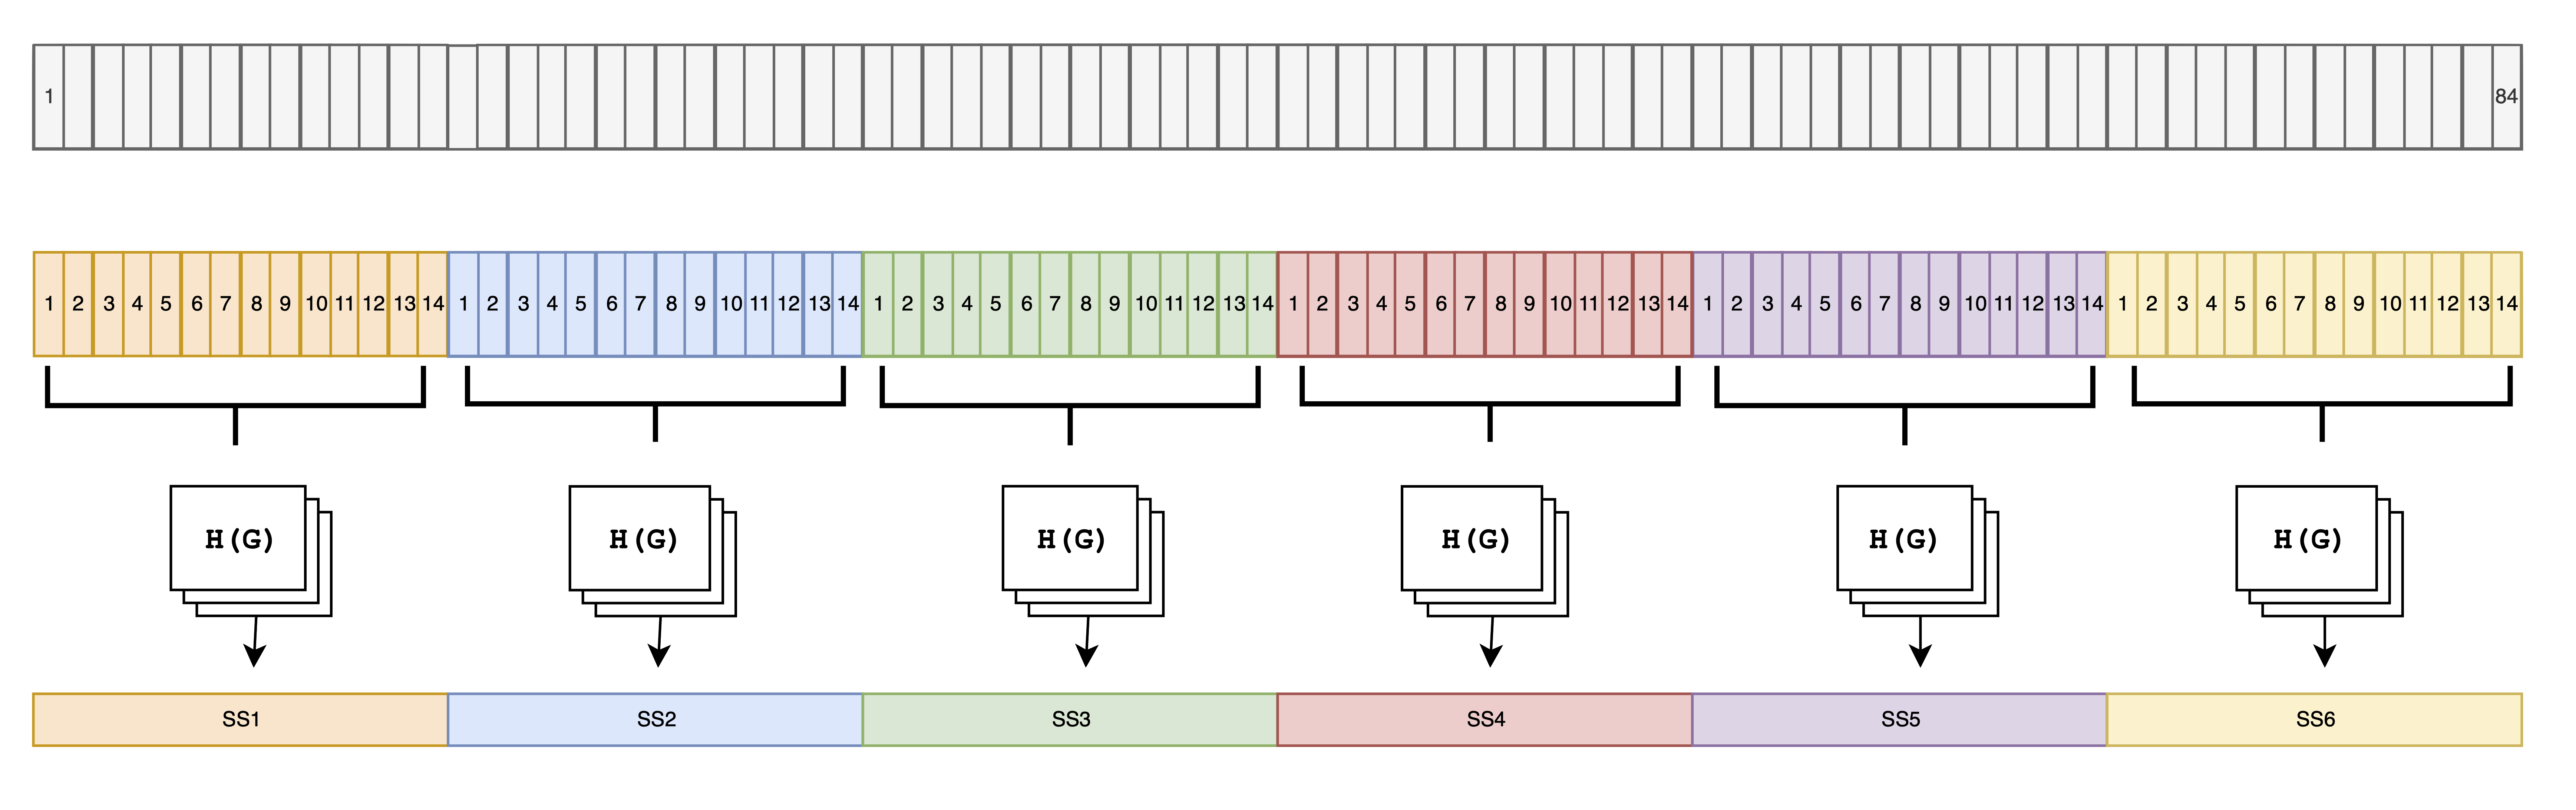
\includegraphics[width=1\textwidth]{Problem3Figs/3image.png}
    \caption{Permutations, Grouping, Re-Hashing into \enquote{Super-sketch}}
    \label{fig:similarity}
\end{figure}
\FloatBarrier

Let's provide some general terminology to accompany this analysis and further ones.  I will call original \textbf{sketch values} $\boxed{\mathbf{v_i}}$ with $1 \leq i \leq 84$ as we have $84$ original values in our sketch.  \textbf{Groups of 14} $v_i$ will be labeled $\boxed{\mathbf{G_j}}$, with $1 \leq j \leq 6$ as we have $6$ groups after segmentation of original sketch values.  The hash function which takes a group value as an input, $\boxed{\mathbf{H(G_j)}}$, will return a super-sketch 64-bit value $\boxed{\mathbf{SS_j}}$ again with $1 \leq j \leq 6$ as we hash $6$ times---once per group.

\subsection{\textit{Super-sketch} Value Matches} \label{section:ssmatch}
It is, of course, true that if a group (1-14) of a document's original sketch values match those of another document, their respective \textit{super-sketch} values will agree as the same amalgamated 14 original sketch values were placed into a hash function, $H(G)$, which will return the same output for two runs on the same input.  This said, we question whether the reverse is true.  Do two matching \textit{super-sketch} values imply that the hash function's output-generating-\textbf{input} of 14 values match in each document:
\begin{align}
    G_{j,a} = G_{j,b} \implies H(G_{j,a}) = SS_{j,a} = H(G_{j,b}) = SS_{j,b}\\
    SS_{j,a} = SS_{j,b} \overset{?}{\implies} G_{j,a} = G_{j,b}
\end{align}

The reverse is not obviously true (in fact, it is not true).  \textbf{However,} given a 64-bit hash-value with a hashing scheme that is seemingly random, we know that the likelihood of two values matching is $\frac{1}{2^{64}}$.  Because this is a negligible likelihood, we can assume:
$$SS_{j,a} = SS_{j,b} \implies G_{j,a} = G_{j,b}$$


\subsection{Two or More \textit{Super-sketches} Match}
We now seek to determine the probability---given resemblance, $r$---that two or more of the 64-bit \textit{super-sketch} values, $SS_j$, match for two documents.  The probability is conditional on $r$:
\begin{align}\label{eq:GoalProbability}
    P(\text{two or more } SS_{j,a} = SS_{j,b} \mid R = r)
\end{align}

To begin our determination of matching \textit{super-sketches} conditional on $r$, we must find a probability more closely linked to $r$.  Resemblance, as defined in the lecture notes, tells the probability an original sketch value in a document matches another.  Using our established notation above:
\begin{align}\label{eq:resemblance}
    P(v_{i,a} = v_{i,b}) = r
\end{align}

Unfortunately, our $SS_j$ 64-bit values depend only on the amalgam group values, $G_j$, and as determined in Section \ref{section:ssmatch}: $G_{j,a} = G_{j,b} \implies SS_{j,a} = SS_{j,b}$.  Conveniently, we can determine the probability $G_{j,a} = G_{j,b}$, as each of the groups' sub-components, $v_{i,a}$ and $v_{i,b}$, is independent and likely to match with probability $r$.

\textbf{Probability a $\mathbf{G_{j,a} = G_{j,b}}$}:
\begin{align}
    P(G_{j,a} = G_{j,b}) = P(v_{1,a} = v_{1,b} \cap v_{2,a} = v_{2,b} \cap ... \cap v_{14,a} = v_{14,b}) = r^{14}
\end{align}

Now, we are ready to determine the probability that two \textit{super-sketch} values might agree.  Though previously we stated $SS_{j,a} = SS_{j,b} \implies G_{j,a} = G_{j,b}$, because the previously claimed \enquote{negligible} probability of a collision was $\frac{1}{2^{64}}$, I will not take for granted this assumption, as we intend to change the bit-width of the final hash output.  Instead, using conditional and total probability, we can better model the situation.

\textbf{Probability a \textit{super-sketch} agrees}: 
\begin{align}
    P(SS_{j,a} = SS_{j,b}) &= \underbrace{P(SS_{j,a} = SS_{j,b} \mid P(G_{j,a} = G_{j,b})}_{1} \underbrace{P(G_{j,a} = G_{j,b})}_{r^{14}}\ \mathbf{+} \ \underbrace{P(SS_{j,a} = SS_{j,b} \mid P(G_{j,a} \neq G_{j,b})}_{\frac{1}{2^{64}}} \underbrace{P(G_{j,a} = G_{j,b})}_{1 - r^{14}}
\end{align}
\begin{align} \label{eq:agree}
    P(SS_{j,a} &= SS_{j,b}) = r^{14} + \frac{1-r^{14}}{2^{64}}
\end{align}

From here we will refer to the probability that a \textit{super-sketch} agrees across two documents (Equation \ref{eq:agree}) as $\boxed{\mathbf{P_{agree}}}$.\\

\textbf{Probability two or more \textit{super-sketches} agree (given $r$)}: 
Now, we are ready to return to Equation \ref{eq:GoalProbability}.  To find the probability that 2 or more \textit{super-sketch} values agree across two documents, we can find the probabilities that none or only 1 \textit{super-sketch} value pair agrees across documents and take the complement:
\begin{align}
    P(\text{two or more } SS_{j,a} = SS_{j,b}) &= 1 - \left [ {6 \choose 0} (1-P_{agree})^6 + {6 \choose 1}P_{agree}(1-P_{agree})^5 \right] \\
    P(\text{two or more } SS_{j,a} = SS_{j,b}) &= 1 - \left[ \left (1 - r^{14} - \frac{1 - r^{14}}{2^{64}}\right )^6 + 6\left (r^{14} + \frac{1 - r^{14}}{2^{64}}\right )\left (1 - r^{14} - \frac{1 - r^{14}}{2^{64}}\right )^5\right]
\end{align}

\begin{figure}[h!]
    \centering
    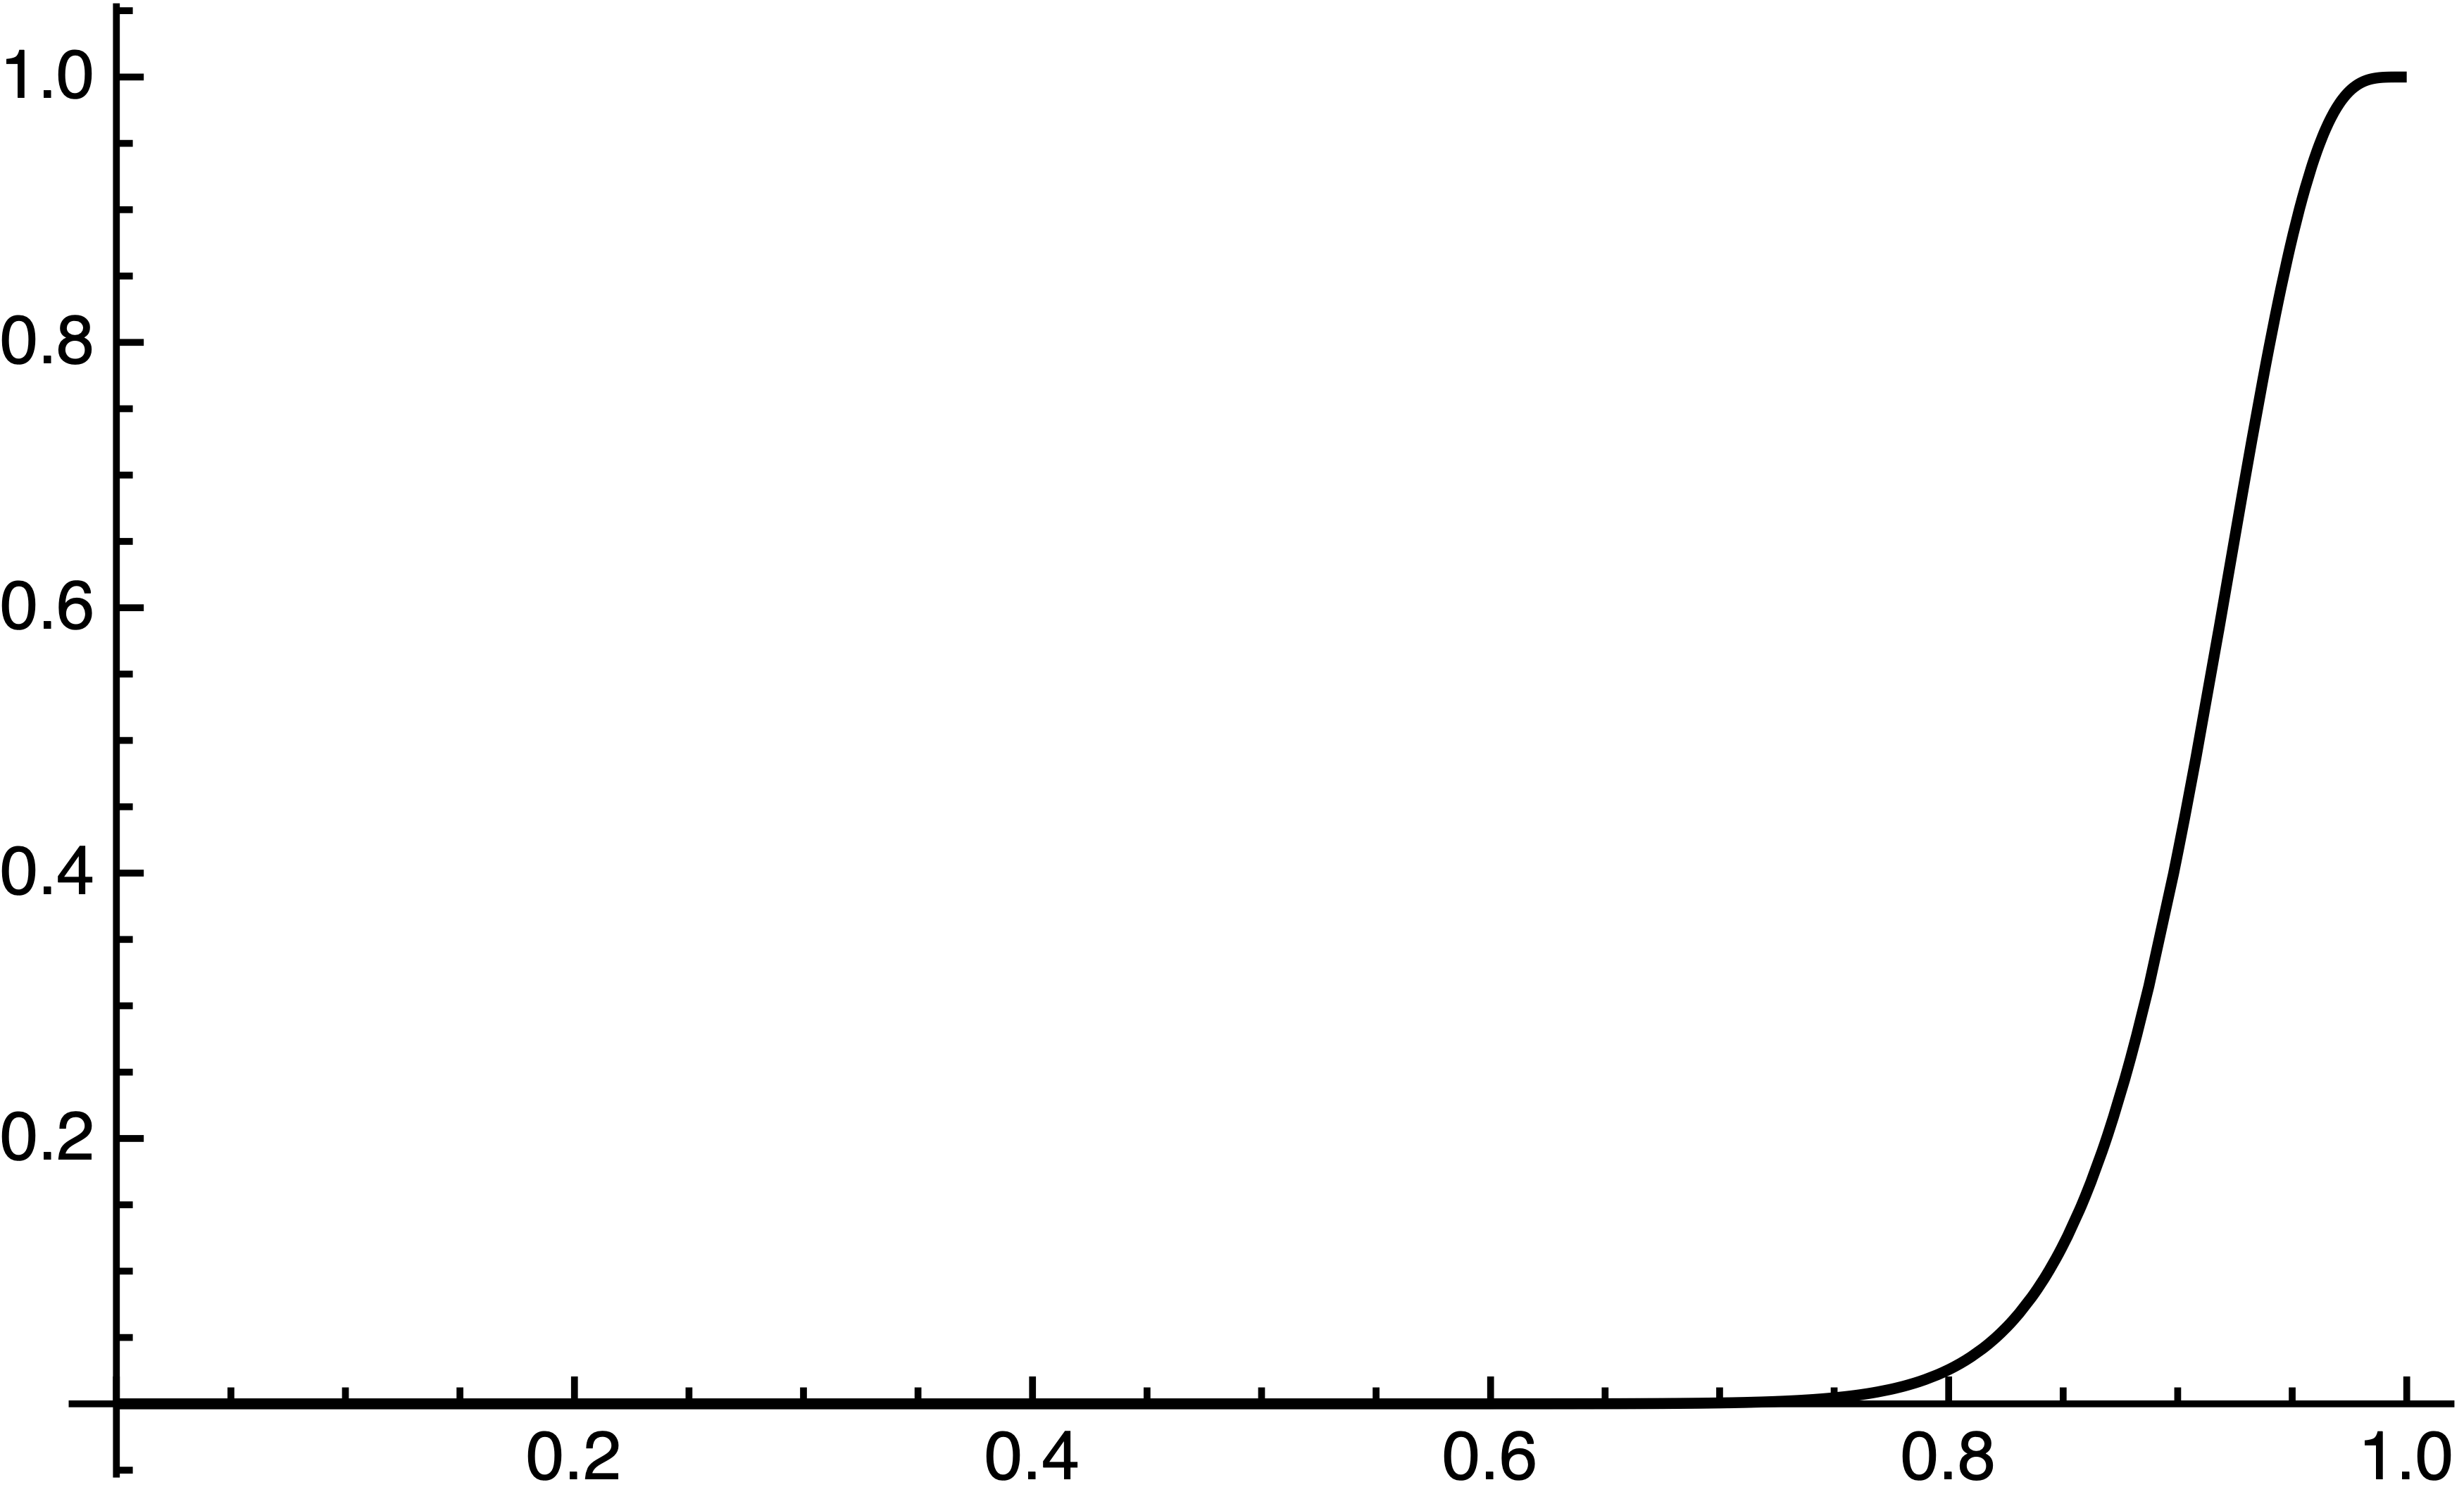
\includegraphics[width=0.65\textwidth]{Problem3Figs/64-bit.png}
    \caption{Probability two or more \textit{super-sketches} agree v. $r$}
    \label{fig:64-bit}
\end{figure}
\FloatBarrier

Much like in lecture with 100 values kept in the calling card, our \textit{super-sketch} methodology preserves a high cut-off for resemblance, ensuring even just for two matches (what's plotted again is the probability of two or more matches) that the probability is low until resemblance is quite high!


\subsection{Varying hash bit-width}
\begin{figure}[h!]
    \centering
    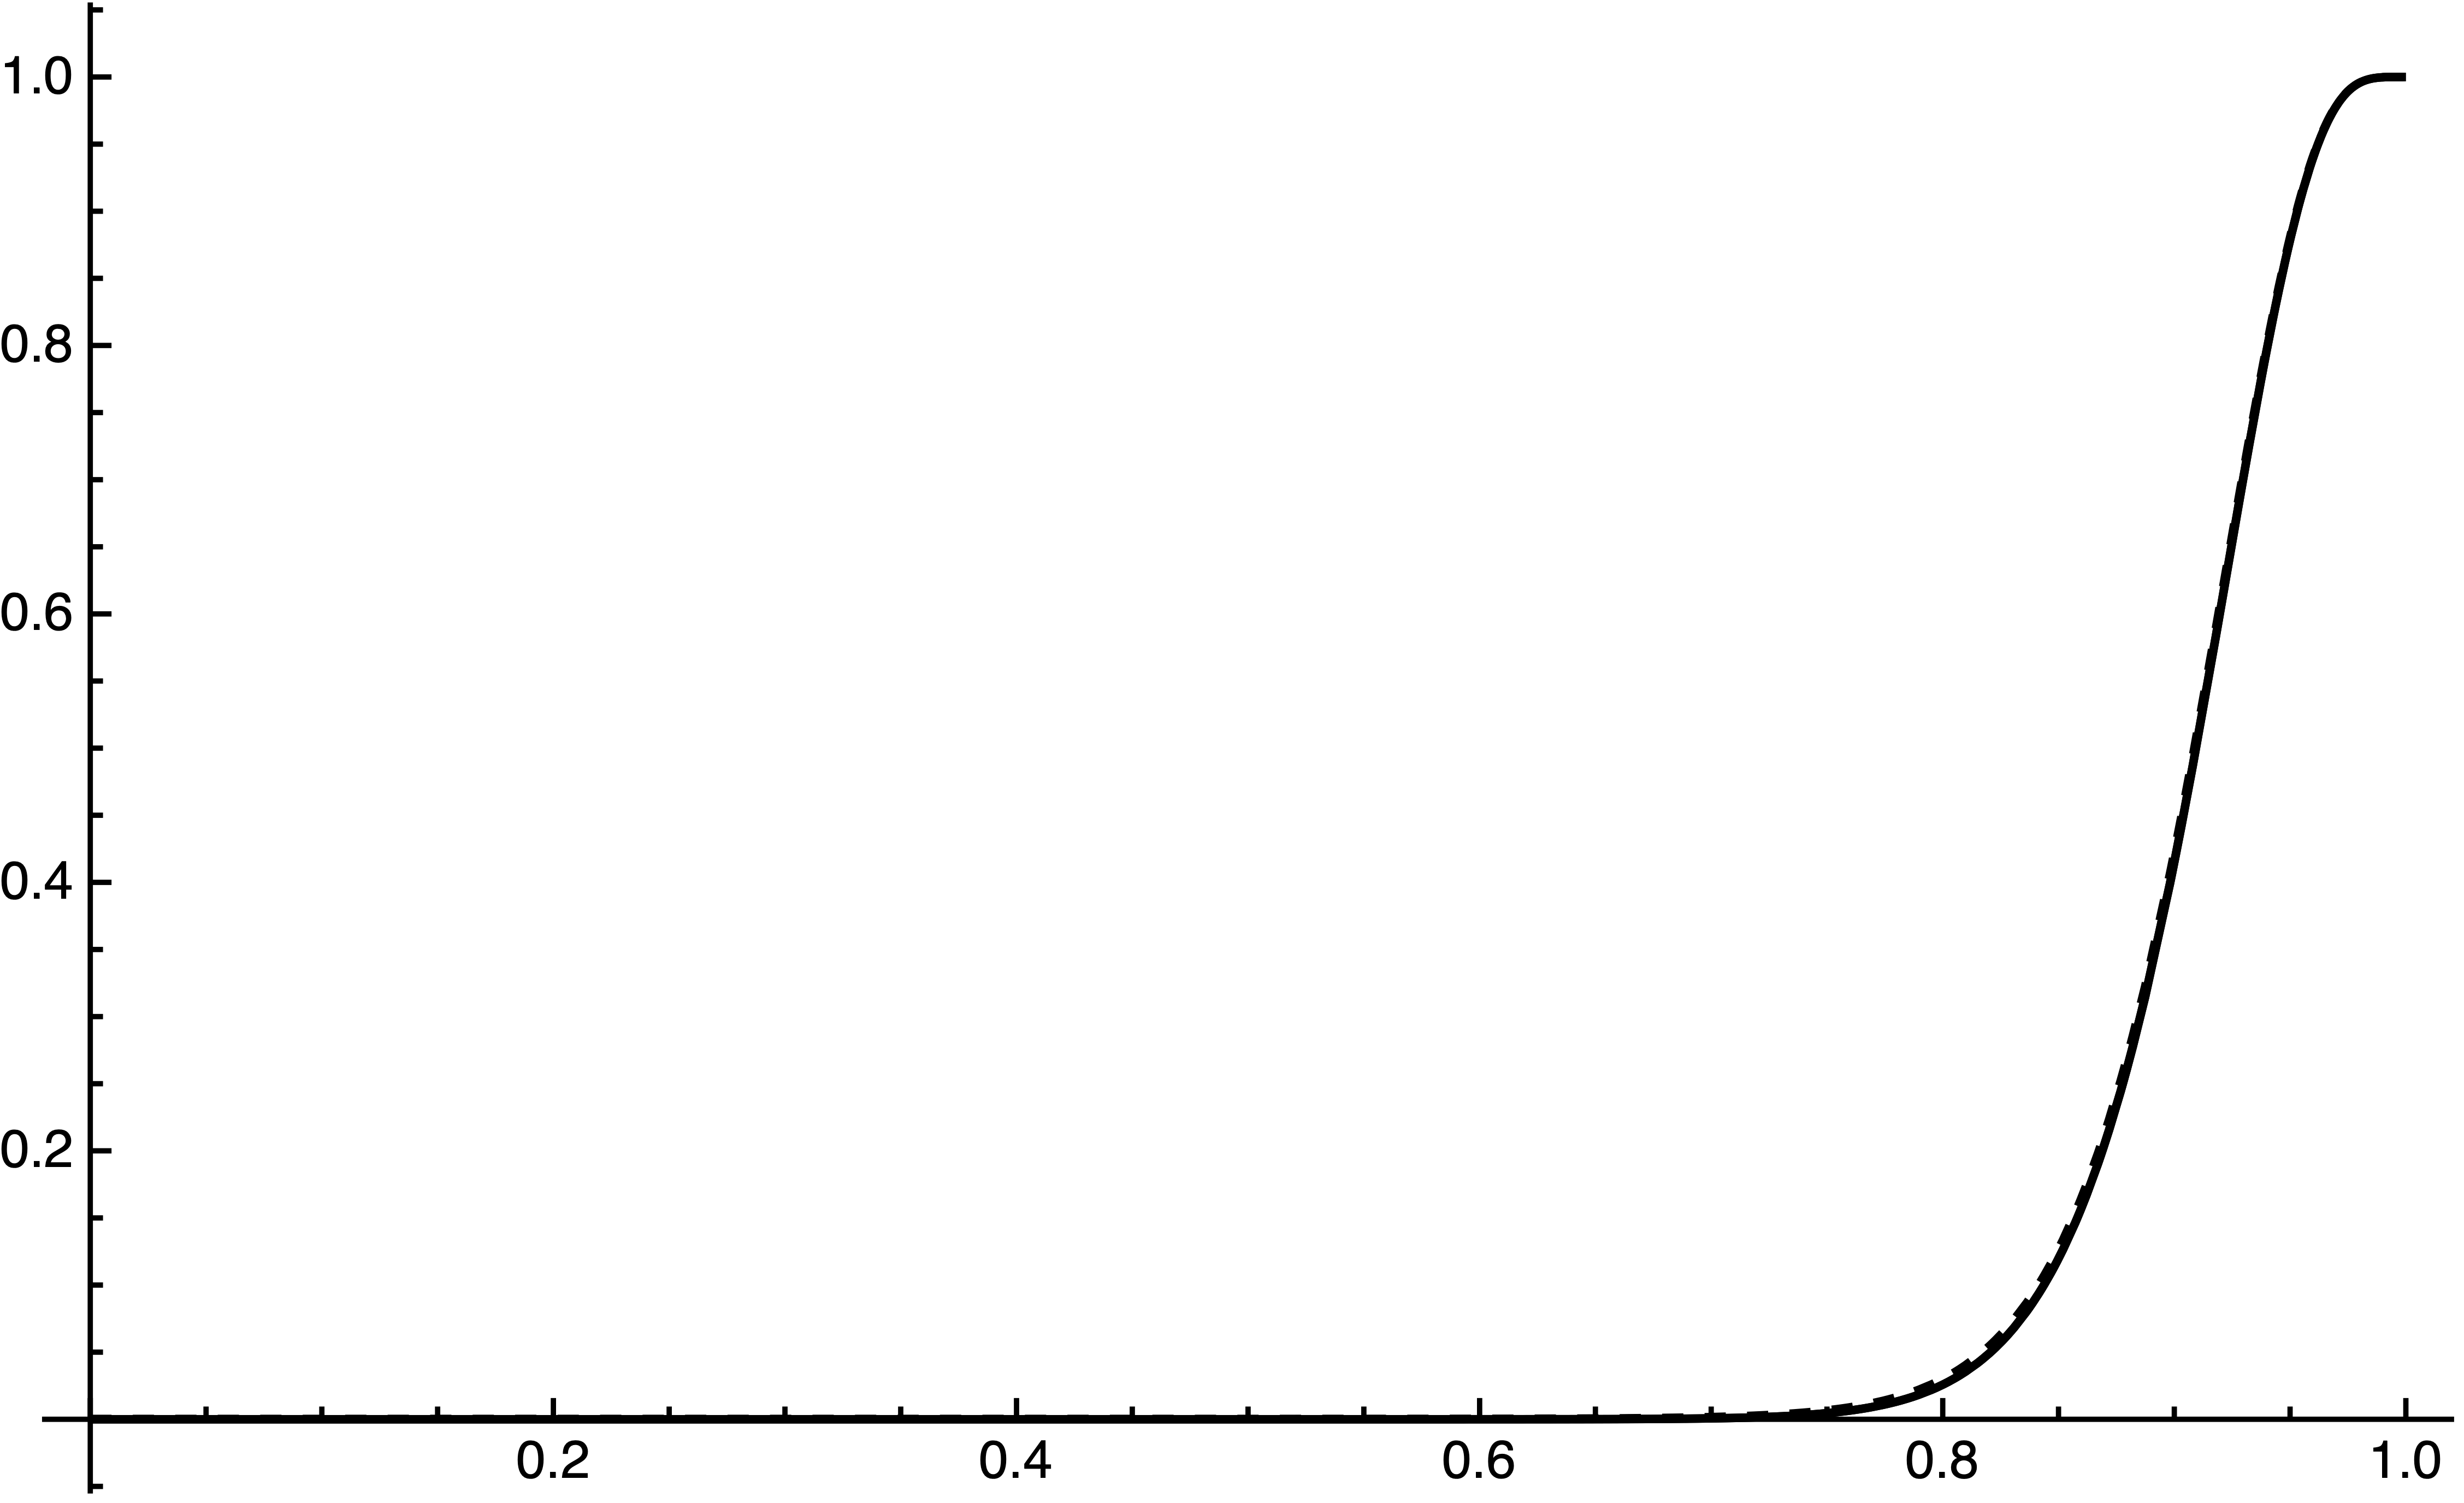
\includegraphics[width=0.65\textwidth]{Problem3Figs/comparison.png}
    \caption{8,16,64-bit Hash and Probability two or more \textit{super-sketches} agree v. $r$}
    \label{fig:comparison}
\end{figure}
\FloatBarrier
At resemblance, $r = 0.8$, there was a $0.005$ difference in probability between the 8-bit (higher probability) and 16-bit hashes.  At scale, this difference \textit{may} be meaningful, but at a cursory glance, the differences are negligible and the graphs look similar and indistinguishable to the eye.  On Figure \ref{fig:comparison} above, the nearly indiscernible dashed line represents the 8-bit configuration which only slightly deviates from the curve for the 16 and 64-bit hashes (completely indiscernible).

\newpage

\section{Composites + RSA}
%%%%%%%%%%%%%%%%%%
%   Question #4  %
%%%%%%%%%%%%%%%%%%

\subsection{636127 is composite}
From section notes, we are provided an algorithmic way to identify a \textit{witness} and prove composite-ness:  For a prime candidate, $n$, let $u$ be such that $n-1 = 2^t u$.  For some $a$, calculate $a^u$.  \textbf{If} at any time we have $a^{2^{i-1} u} \neq \pm 1\  \text{mod}\  n$ \textbf{and} $a^{2^i u} \equiv 1\  \text{mod}\  n$, \textbf{then} we have a non-trivial square root. \\

It is most sensible to approach the task of finding a \textit{witness} through a script to solve the problem.

\rule{\textwidth}{0.4pt}
$$\mathbf{636127} \textbf{ is composite} \text{ with } \textit{witness}: \mathbf{476323}$$
\rule{\textwidth}{0.4pt}

\textbf{Note:} When finding the witness, I first choose the largest possible $t$ thereby minimizing $u$.  Then I select a random base, $a$, within [2, $n-1$] and choose $i = 1$ such that I can show the following: 
\begin{align}
    a^{2u} \equiv 1\  \text{mod}\  n \\
    a^{u} \nequiv \pm 1\  \text{mod}\  n
\end{align}

In finding a \textit{witness} for $636127$, I found largest $t = 1 \implies u = 318063$.

\subsection{294409 is composite}
In finding a \textit{witness} for $294409$, I found largest $t = 3 \implies u = 36801$.\\

\rule{\textwidth}{0.4pt}
$$\mathbf{294409} \textbf{ is composite} \text{ with } \textit{witness}: \mathbf{145653}$$
\rule{\textwidth}{0.4pt}

Fermat's Little Theorem (FLT) will not help here for the Carmichael number, $294409$.  Though $294409$ is an $145653$-pseudoprime (i.e., $145653^{294409-1} \text{ mod } 294409 = 1$), we are not guaranteed that $294409$ is prime---it actually is factorable (109, 73, 37)---and $294409$ will be an $a$-pseudoprime for any choice of $a$ relatively prime to $294409$.



\subsection{RSA Encoding: Give me an A}
To encrypt the message \enquote{Give me an A} as if it were to be sent to Michael Mitzenmacher using his public RSA key---provided (n,e)---I first converted the ASCII string to it's binary equivalent, appending each 8-bits as I parsed the sentence for characters.  (See more in Section \ref{CODE: RSA}.)  This binary value, I then converted to decimal form (technically, in the code, I converted to decimal each step of parsing, but it's easier to explain the other way).  Using the standard method:
\begin{align*}
    \textbf{Message in decimal: } & m\\
    \textbf{Encrypted message: } & e(x) = m^e\ \text{mod}\ n
\end{align*}

\rule{\textwidth}{0.4pt}
$$e(x) = 27016764340118192395712492378$$
\rule{\textwidth}{0.4pt}

\subsection{Code Excerpts}
\subsubsection{4A/B: Witness Finding}
\begin{minted}{python}
## 4a/b: find a witness ##

import math
from random import seed
from random import randint



# seed random number generator
seed(124) # heh, 124

# prime candidate
n = 636127 # or 294409

# let u be such that n-1 = u * 2^t
def highestPowerOf2(n):  
    return (n & (~(n - 1))) 

t = int(math.log2(highestPowerOf2(n-1)))
print(f"Finding smallest u, use t = {t}")

u = int((n-1)/(2**t))
print(f"u = {u}\n")

success = 0;

while True:
    # pick random "a" (witness) [restrict range to nontrivial cases]
    a = randint(2, n-2)
    
    # pow(x,y,z) returns x**y % z

    ## satisfy first case with i = 1: a^((2^i)*u) % n = 1 % n = a^(2u) % n
    lhs = pow(a, 2*u, n)
    if lhs == (1 % n):
        print(f"Preliminary success with witness {a}")

        ## satisfy second case with i = 1: a^((2^(i-1))*u) % n =  1 % n = a^(u) % n
        stepTwo = pow(a, u, n)
        if stepTwo != (1%n) or stepTwo != (-1 % n):
            print(f"GREAT SUCCESS with witness a = {a}\n")
            break;
\end{minted}

\subsubsection{RSA for Mitzenmacher} \label{CODE: RSA}
\begin{minted}{python}
## convert ASCII to binary to decimal
original = "Give me an A"
segments = list(original)

len_list = len(segments)
decimalMessage = 0

for i in range (0, len_list):
  decimalMessage += ord(segments[i]) * 2**((len_list-i-1)*8)

# Mitzenmacher RSA Public Key
n,e = 46947848749720430529628739081, 37267486263679235062064536973

e_x = pow(decimalMessage, e, n)
\end{minted}














\newpage

\section{Bins, Balls, Billions}
\subsection{Non-sequential}
\textbf{Methodology:}\\
I model the throwing of 1 billion balls into 1 billion bins (uniform, random, independent) in the following way:
\begin{enumerate}
    \item As Prof. M suggested, I keep track of an array, $A[i]$, which represents the number of bins with $i$ balls
    \item I also keep track of the number of non-empty bins (i.e., $\text{Total Bins} - A[0]$)
    \item On the first iteration of my ball tossing, I simply initialize $A[1] = 1$ thereby containing 1 bin (as a ball must enter a bin $\implies$ 1 bin has 1 ball---all others empty).
    \item On subsequent tosses, I randomly generate a bin number and \textbf{if} the number is strictly greater than the number of non-empty bins, I make it a \enquote{new} bin by decrementing from the empty bins index, $A[0]$, and incrementing the 1-ball-in-bin index, $A[1]$ (also incrementing the number of non-empty bins---yes this is redundant).  \textbf{Else}, the generated bin number is less than or equal to the number of non-empty bins, so I find the bin corresponding to this bin number by iterating through the array until I find the index where the bin would exist (see diagram below for details), and I move the bin to the next index of $A$, indicating that I added a ball to the bin.
\end{enumerate}

I assert that this method retains generality in view of probabilistic integrity. \\

\textbf{Methodology (by example):}  Suppose I intend to place 10 balls into 10 bins.  Below, I show my array, $A$, and the method by which I adjust its elements:
\begin{figure}[h!]
    \centering
    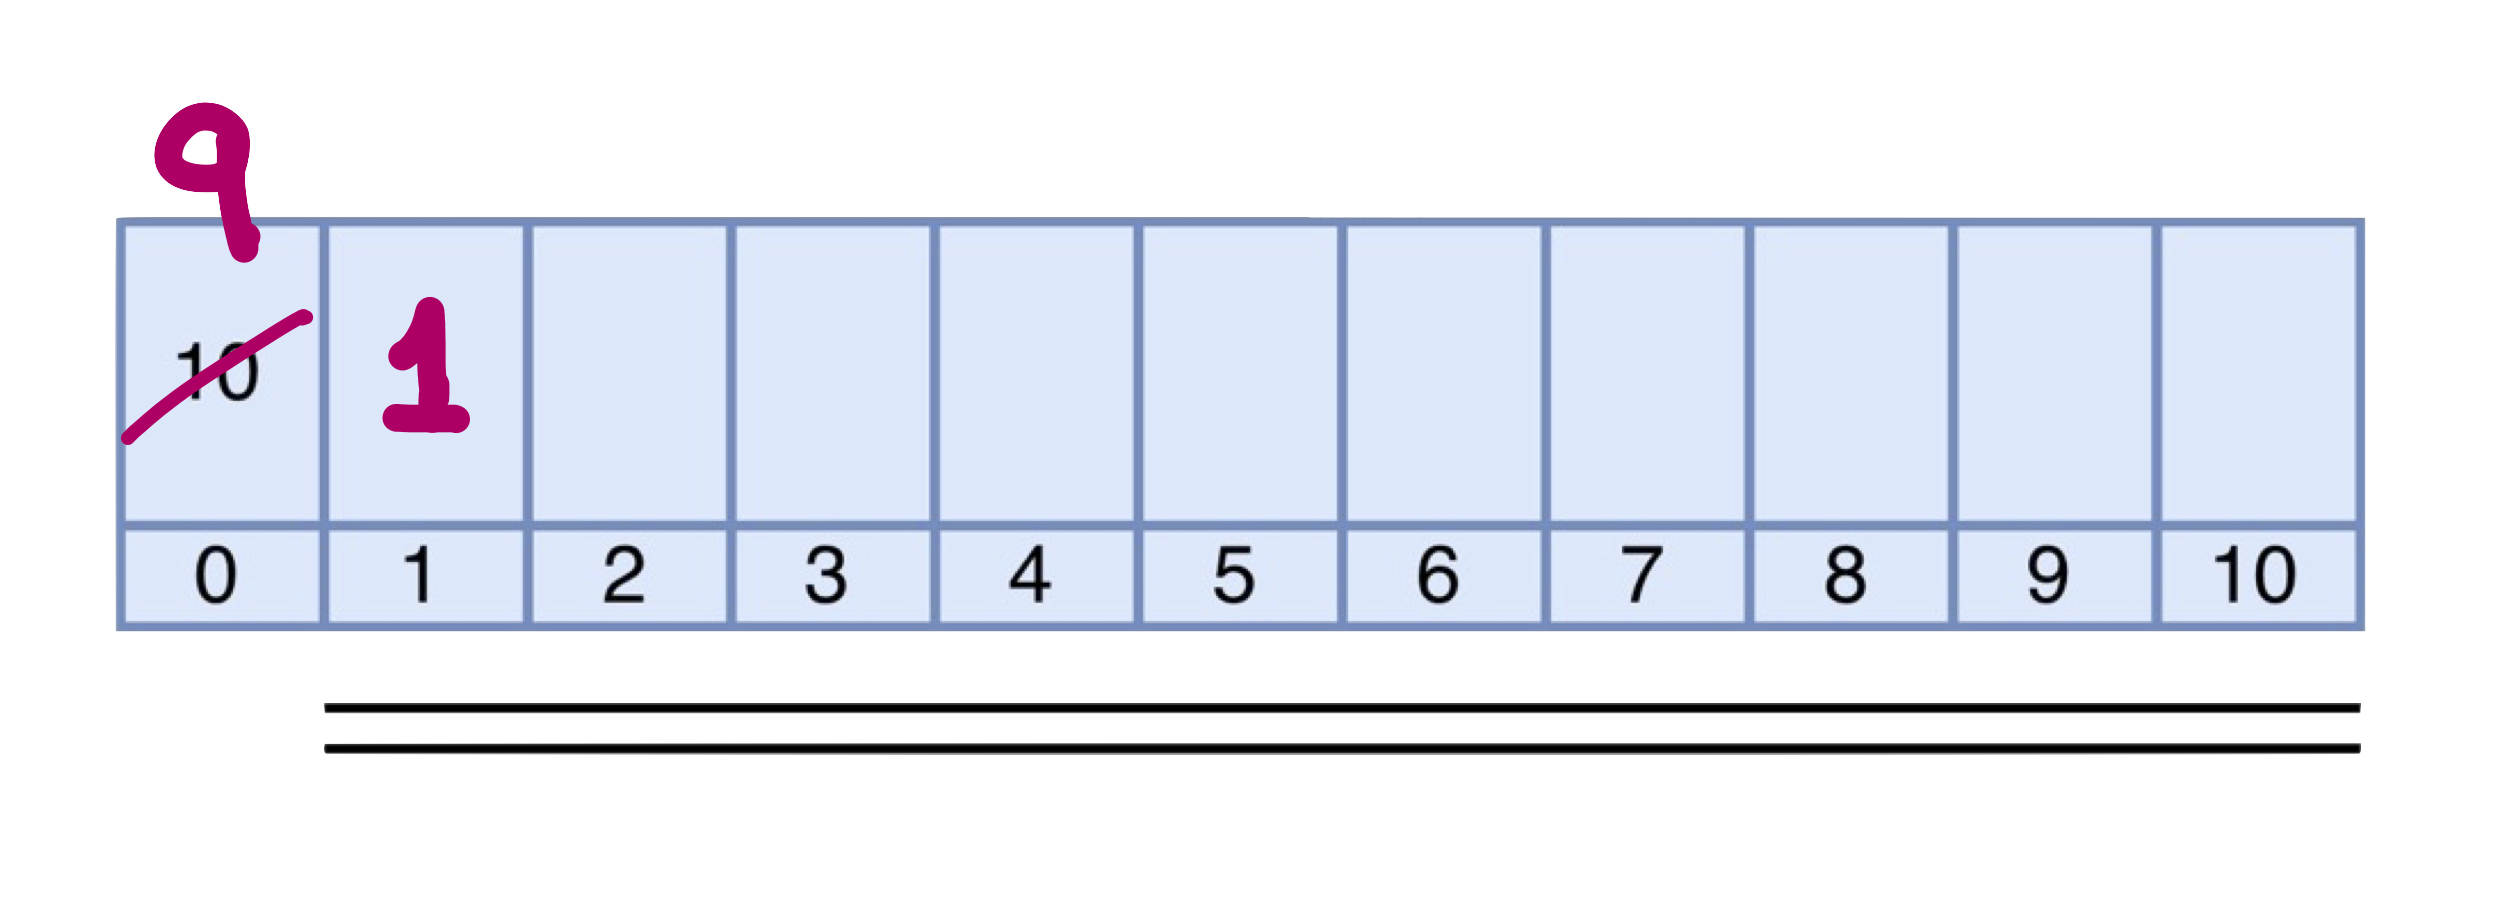
\includegraphics[width=0.45\textwidth]{Problem5.1Figures/start.png}
    \caption{Initialization and Iteration 1}
    \label{fig:start}
\end{figure}
\FloatBarrier

First, I place all of my bins in $A[0]$ as they are all empty (have no balls).  Then on my first iteration, I throw a ball in a bin (doesn't matter which), so I now have 1 bin with 1 ball and 9 bins with 0 balls as seen in Figure \ref{fig:start}.

\begin{figure}[h!]
    \centering
    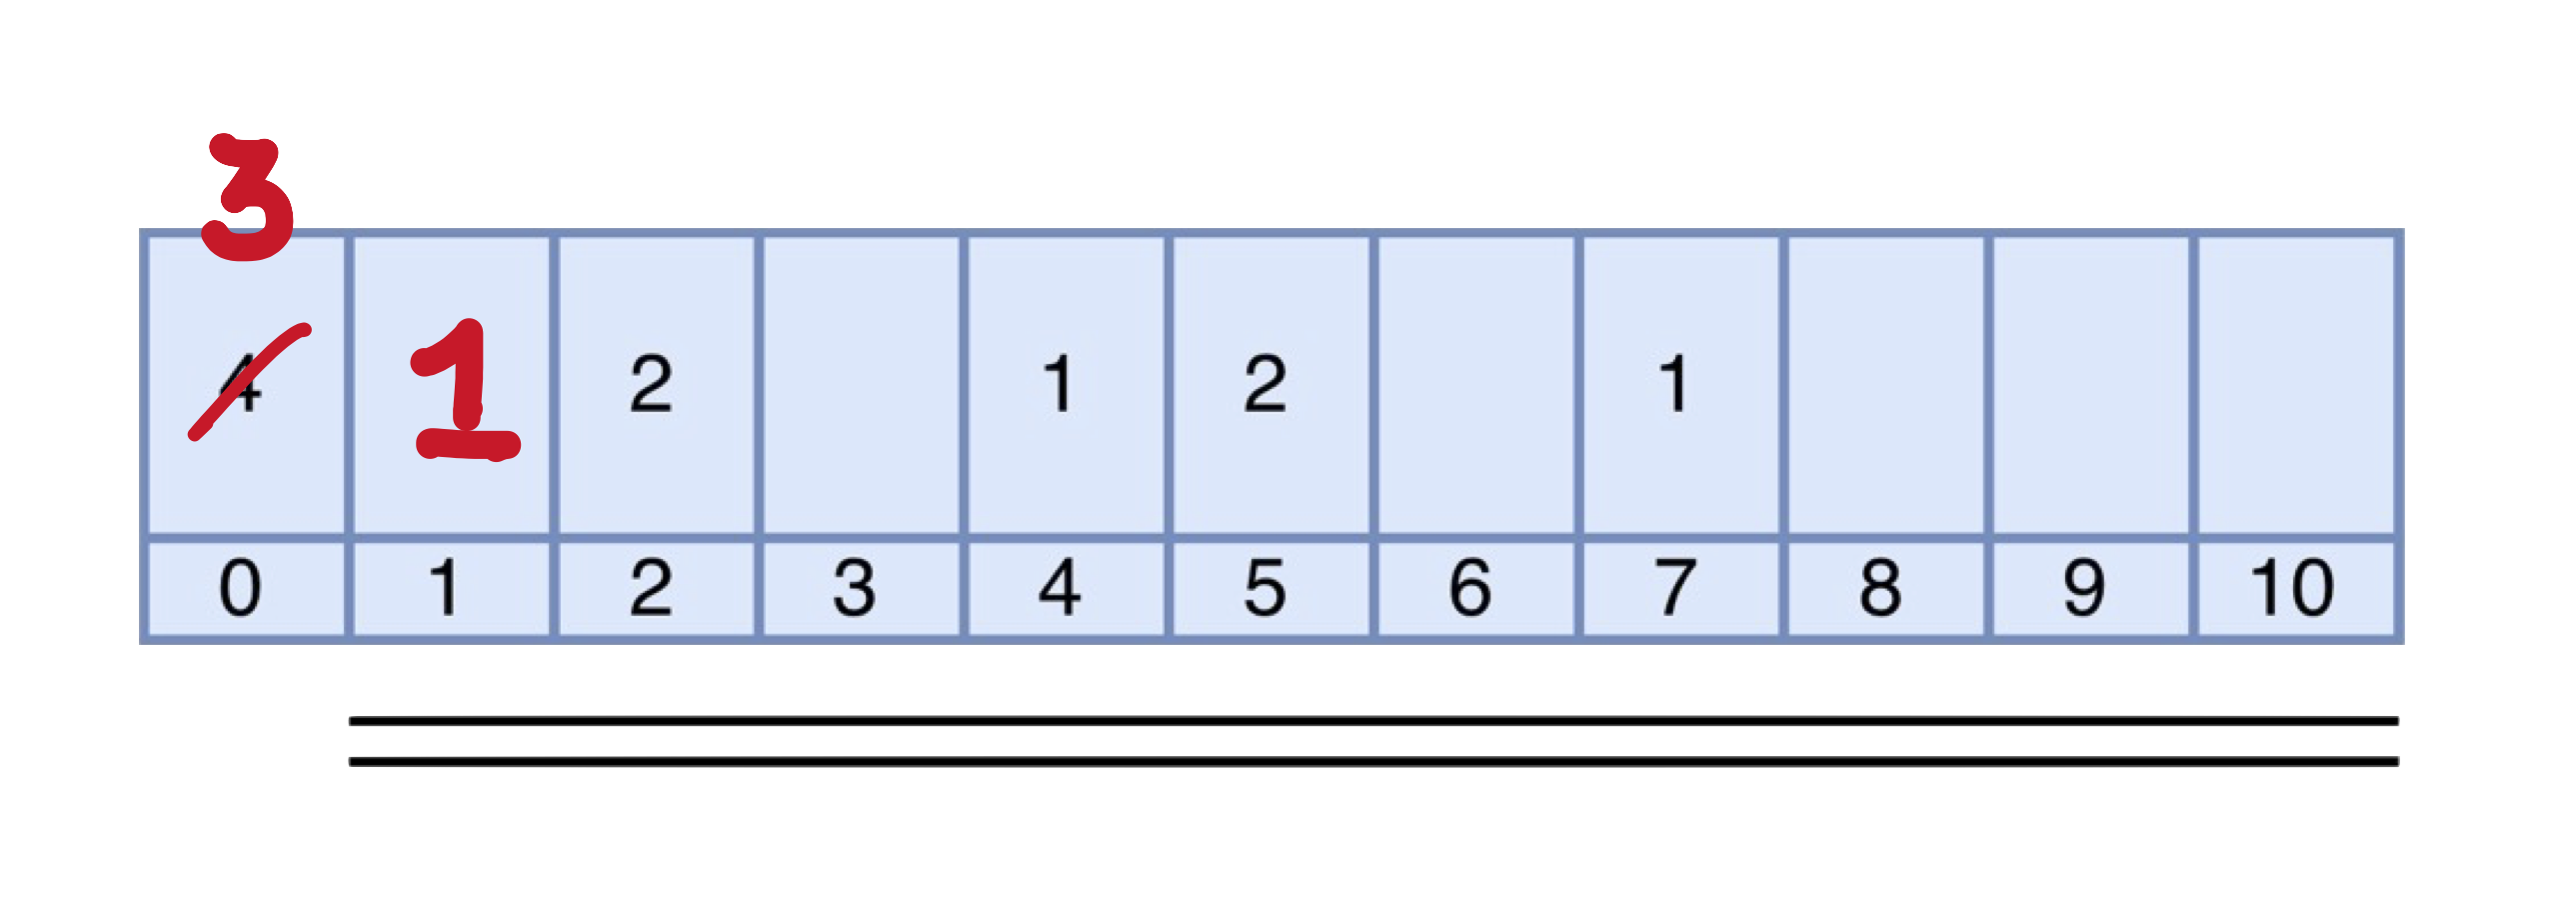
\includegraphics[width=0.45\textwidth]{Problem5.1Figures/scenario2.png}
    \caption{Iteration 7, randomly selected bin number > $\sum_{i=1}^{10} A[i]$}
    \label{fig:scenario1}
\end{figure}
\FloatBarrier

Next, suppose I generate a bin number and it happens to be \textit{greater than} the number of non-empty bins (represented by $10 - A[0]$ or $\sum_{i=1}^{10} A[i]$).  I treat this bin, then, as a \enquote{new} bin, removing an empty bin, and incrementing $A[1]$ to show the new bin with 1 freshly placed ball in it.


\begin{figure}[h!]
    \centering
    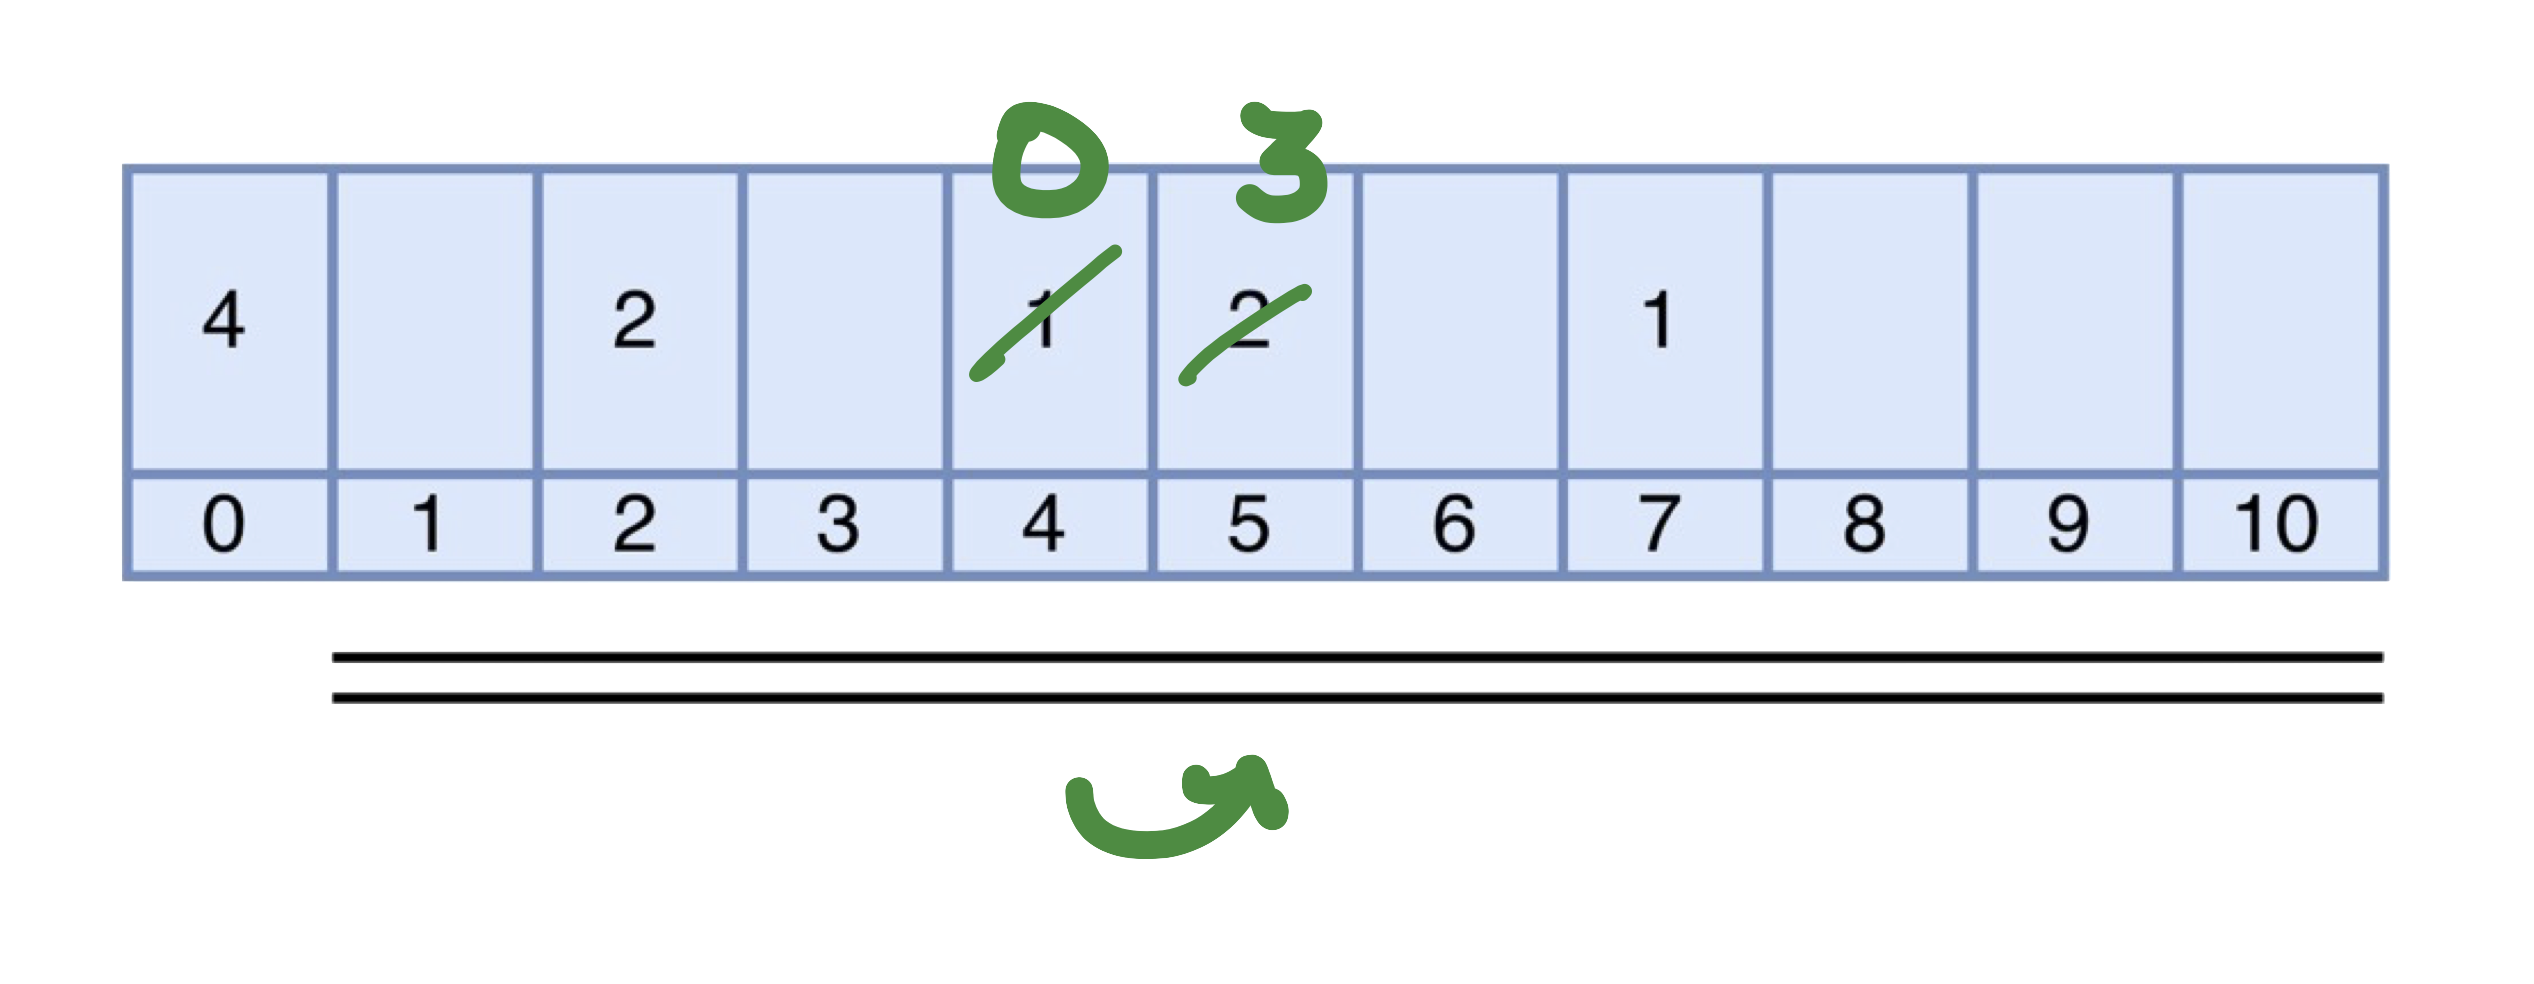
\includegraphics[width=0.45\textwidth]{Problem5.1Figures/scenario1.png}
    \caption{Iteration 7, randomly selected bin number = 3 $\leq$ $\sum_{i=1}^{10} A[i]$}
    \label{fig:scenario2}
\end{figure}
\FloatBarrier

Now, suppose I had generated a bin number and it happened to be \textit{less than or equal to} the number of non-empty bins (represented by $10 - A[0]$ or $\sum_{i=1}^{10} A[i]$).  I treat this bin, then, as an \textit{existing} bin.  I \enquote{search} for the selected bin by walking through my array, $A$, incrementing an iterator with each bin counted at each index in $A$ until my iterator equals the bin number for which we are searching.  At this point, I note the index $i$ of $A$ at which the iterator matched the selected bin (\textbf{the iterator is not equivalent to the index $i$ of $A$} as seen in the example above), and I transfer one bin from $A[i]$ to $A[i+1]$. \\

\textbf{Results:}
\begin{table}[htbp]
  \centering
    \begin{tabular}{l||r|r|r}
    \textbf{Max Load} & 11    & 12    & 13 \\
    \textbf{Frequency} & 44    & 50    & 6 \\
    \end{tabular}%
  \caption{Findings from 100 Trials, 1B Balls \& Bins}
  \label{tab:BallsBins1}%
  \textbf{Average maximal load} = \textbf{11.62}
\end{table}%



\subsection{Sequential (Least-loaded)}
\textbf{Methodology:}\\
Here, I amended my simulation such that it generates two bin numbers (random, uniform), and determines the lesser-loaded of the two bins.  In practice, I check to see if both numbers generated are less than or equal to the number of non-empty bins (in which case, the generated numbers would correspond to a bin with 1+ balls in it).  If this is the case, I choose the lower of the two generated bin numbers---after all, in my searching mechanism, the lower number will deterministically correspond to an index $i$ in $A$ which is lower than (or equal to) that of the larger randomly generated bin number---and fill the corresponding bin.  If \textit{either} of the two randomly generated bin numbers is larger than the number of non-empty bins, one or both bin numbers point to an empty bin $\implies$ all we need to change is increment our non-empty bin count, decrement $A[0]$ (empty bins), and increment $A[1]$ (bins with 1 ball).\\

\textbf{Results:}
\begin{table}[h!]
  \centering
    \begin{tabular}{r||c}
    \textbf{Max Load} & 4 \\
    \textbf{Frequency} & 100 \\
    \end{tabular}%
  \caption{Findings from 100 Trials, 1B Balls \& Bins}
      The results converge such that \textbf{maximal load} = \textbf{4}
  \label{tab:BallsBins2}%
\end{table}
\FloatBarrier

\subsection{Code Excerpts:}
\textbf{Note:} The non-sequential and sequential trials looked quite similar while retaining generality and probabilistic integrity.  For sequential, I replaced a few lines in \textit{binUpdater()} to find the lesser of two randomly generated integers passed in via the \textit{ball\_sim()} function.  In essence, it followed the same form. \\

\begin{minted}{c++}
#include <stdio.h>
#include <stdlib.h>
#include <stdint.h>
#include <vector>
#include <random>

using namespace std;

// ==================================
// HELPER FUNCTION:
// Finds randomly selected bin
// Updates value of balls in that bin
// ==================================
void binUpdater(int selectedBin, vector<int> &array){
    int iterSum = 0;
    int sizeOfA = array.size();
    int shiftIndex = 1;

    // for all non-empty bins, find "selectedBin"
    for (int i = 1; i < sizeOfA; i++) {
        iterSum += array[i];

        if (selectedBin <= iterSum) {
            shiftIndex = i;
            break;
        }
    }

    // now move a bin from this shiftIndex to the next
    if ((shiftIndex + 1) < sizeOfA) {
        array[shiftIndex] -= 1;
        array[shiftIndex + 1] += 1;
    }
    else {
        array[shiftIndex] -= 1;
        array.push_back(1);
    }
}

// ==================================
// Main Simulation:
// ==================================
int balls_sim(int binsAndBalls) {
    
    // Let's begin by creating our A array having all bins with 0 balls in them
    // create 2 element array 
    // (total balls at index 0 and 0 balls at index 1 
    // (no bins have 1 ball in it yet))
    // vector<int> name(size, defaultValue)
    vector<int> A (2, 0);
    A[0] = binsAndBalls;

    // Keep running sum over A from i = 1 to i = bins (don't include 0th index entries)
    // Could also do this by the following: (binsAndBalls - A[0])
    int nonEmptyBins = 0;

    static random_device seed; 
    static mt19937 generator(seed());  
    random_device seeder
    static uniform_int_distribution<int> dis(1, binsAndBalls);
    
    for (int i = 0; i < binsAndBalls; i++) {
        int randomSelectedBin = dis(generator);

        // see if the Bin # is strictly > nonEmptyBins
        // if so, place in a new bin; else, place in corresponding existing bin

        if (randomSelectedBin > nonEmptyBins) {
            A[0] -= 1;
            A[1] += 1;
            nonEmptyBins += 1;
        }
        else {
            binUpdater(randomSelectedBin, A);
        }
    }

    int maxLoad = A.size() - 1;
    return maxLoad;
}
\end{minted}

\end{document}
